\documentclass[11pt,a4paper]{article}
\usepackage[utf8]{inputenc}
\usepackage{amsmath}
\usepackage{mathtools}
\usepackage{amsfonts}
\usepackage{amssymb}
\usepackage{graphicx}
\usepackage{caption}
\usepackage{subcaption}
\usepackage{comment}
\usepackage{color}
\usepackage{enumitem}
\usepackage[left=2cm,right=2cm,top=2cm,bottom=2cm]{geometry}
\usepackage{listings}
\usepackage{color}

\setlength{\jot}{10pt}
 
\definecolor{codegreen}{rgb}{0,0.6,0}
\definecolor{codegray}{rgb}{0.5,0.5,0.5}
\definecolor{codepurple}{rgb}{0.58,0,0.82}
\definecolor{backcolour}{rgb}{0.95,0.95,0.92}
 
\lstdefinestyle{mystyle}{
    backgroundcolor=\color{backcolour},   
    commentstyle=\color{codegreen},
    keywordstyle=\color{magenta},
    numberstyle=\tiny\color{codegray},
    stringstyle=\color{codepurple},
    basicstyle=\footnotesize,
    breakatwhitespace=false,         
    breaklines=true,                 
    captionpos=b,                    
    keepspaces=true,                 
    numbers=left,                    
    numbersep=5pt,                  
    showspaces=false,                
    showstringspaces=false,
    showtabs=false,                  
    tabsize=2
}
 
\lstset{style=mystyle}
\graphicspath{ {./figures/} }
\author{Andrew Teta}
\title{ECEN 4532 - Lab 4: MPEG Audio Signal Processing \\ (MP3)}
\date{March 18, 2019}

\begin{document}

\maketitle

\begin{figure}[ht]
	\centering
	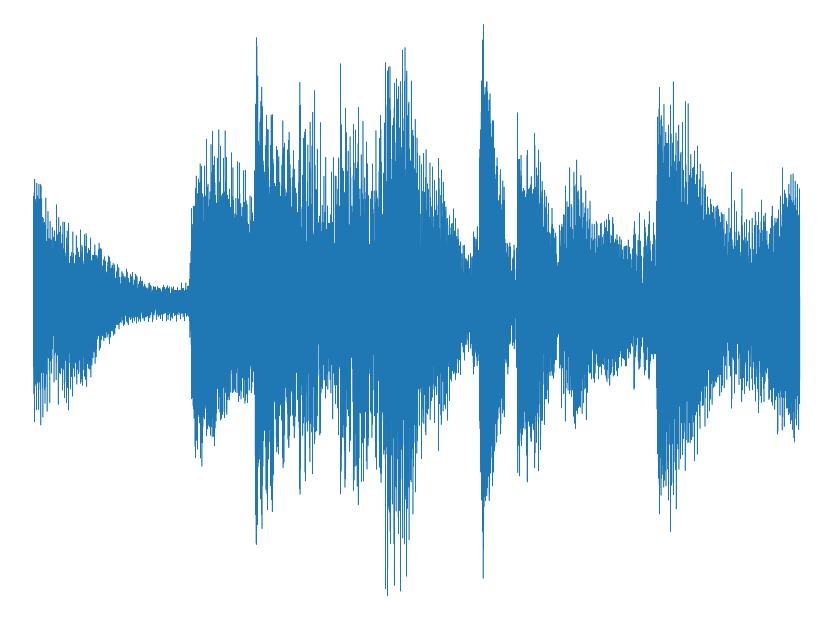
\includegraphics[width=\textwidth]{titlepic}
\end{figure}

\pagebreak

\tableofcontents

\pagebreak

\addcontentsline{toc}{section}{Introduction}
\section{Introduction}
In this lab, we explore signal processing in the context of audio compression. Specifically, we will be constructing the basis of the MPEG 1 Layer III codec, commonly known as MP3. The general idea is to implement a series of sub-band filters to decompose and reconstruct input audio "perfectly" and later, experiment with the exclusion of certain frequency bands as a method of data compression. We will implement the polyphase pseudo-QMF filter bank, which filters the audio signal into 32 frequency bands. The two main procedures in this processing scheme are analysis and synthesis.

\section{Background}
\subsection{Analysis}
Analysis is the process of decomposing a signal into frequency components and filtering it into sub-bands. MP3 encoding splits the audio signal $x(n)$ into 32 equally spaced frequency bands. This is accomplished with 32 parallel filters with impulse response $h_k$ such that,

\begin{equation}
s'_k(n) = h_k(n) * x(n), \quad k = 1, ..., 32.
\end{equation}

By downsampling the output of each filter by a factor of 32, we achieve a critically sampled analysis filter. Thus,

\begin{equation}
s_k(n) = ((h_k * x) \downarrow 32)(n) = s'_k(32n).
\end{equation}

The effect of this procedure (and the idea of critical sampling) is an efficient filter, where for an input block of size $N$ samples of $x(n)$, a total of $N$ output samples are produced.

\subsection{Synthesis}
Reconstruction is performed by upsampling the downsampled signals with zero values and filtering with a synthesis filter bank, $g_k$.

\begin{equation}
s_k \uparrow 32) * g_k(n), \quad k = 1, ..., 32.
\end{equation}

The synthesized output, $\tilde{x}$ is found by the sum of all the synthesis filters,

\begin{equation}
\tilde{x} = \sum_{k=1}^{32} (s_k \uparrow 32) * g_k(n).
\end{equation}

The MP3 filter bank has nearly (but not exactly) perfect reconstruction and fortunately the error is not an issue. The filter design is greatly simplified by using a prototype filter, modified only slightly for each of the 32 analysis filters, $h_k$.

\pagebreak

\section{Cosine Modulated Pseudo Quadrature Mirror Filter: Analysis}
This section describes the mathematical description of MP3 analysis and further derives a fast algorithm to compute both convolution and decimation together, producing the output signal $s_k$ for each of the 32 sub-bands.

\subsection{The math}
Consider a 512 tap filter $h_k$ such that

\begin{equation} \label{eq:analysis_output}
s_k(n) = \sum_{m=0}^{511} h_k(m) x(32n - m)
\end{equation}

and

\begin{equation}
h_k(m) = p_0(m) cos\left(\frac{(2k + 1) (m-16) \pi}{64} \right) \quad k = 0, ..., 31, \quad m = 0, ..., 511.
\end{equation}

$p_0$ is a prototype lowpass filter (see Fig. \ref{fig:sinc})and the multiplication with $cos\left(\frac{(2k + 1) (m-16) \pi}{64} \right)$ shifts the center frequency of $p_0$ to be centered around $(2k + 1)\pi/64$. Thus, $h_k$ becomes a bandpass filter, selecting frequencies around $(2k + 1)\pi/64$, for $k=0,...,31$, and a nominal bandwidth of $\pi/32$.

\begin{figure}[ht]
	\centering
	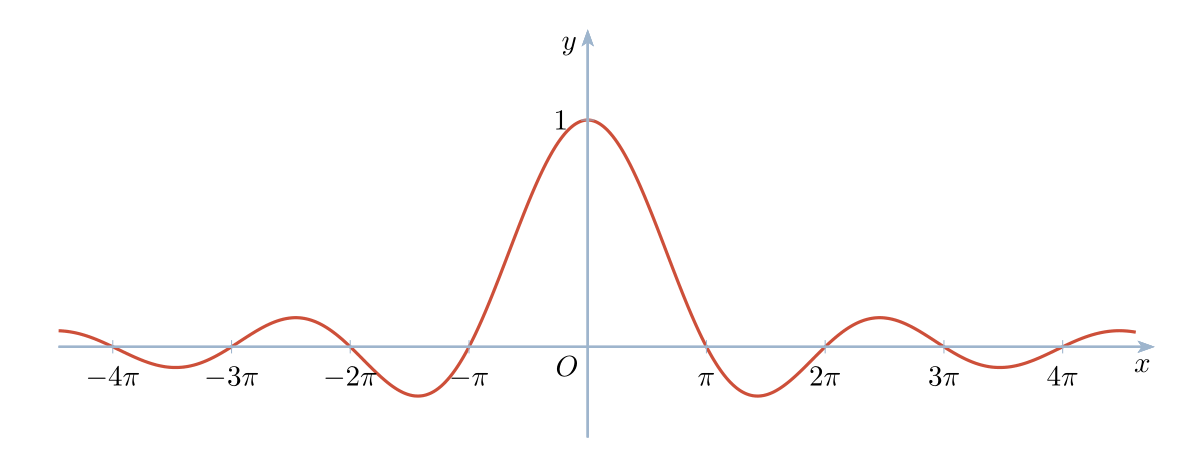
\includegraphics[width=0.6\textwidth]{analysis/sinc}
	\caption{A cartoon representation of $p_0$, the prototype filter used for analysis of a signal in MP3 encoding. This plot has no relevance to scale and is only a reference to the general shape of $p_0$ and its lowpass filter construction.}
	\label{fig:sinc}
\end{figure}

\pagebreak

\subsection{Derivation of a faster way}
We begin with \eqref{eq:analysis_output} and decompose the summation by letting $m=64q + r$

\begin{equation}
s_k(n) = \sum_{m=0}^{511} h_k(m)x(32n - m) = \sum_{q=0}^7 \sum_{r=0}^{63} h_k(64q + r)x(32n - 64q - r)
\end{equation}

and since

\begin{equation}
h_k(m) = p_0(m)cos\left(\frac{(2k + 1) (m - 16)\pi}{64} \right),
\end{equation}

we can write

\begin{align}
h_k(64q + r) &= p_0(64q + r)cos\left(\frac{(2k + 1) (64q - r - 16)\pi}{64} \right) \\
			&= p_0(64q + r)cos\left(\frac{(2k + 1) (r - 16)\pi}{64} + (2k + 1)q\pi \right) \\
			&= 
			\begin{dcases}
				p_0(64q+r)cos\left(\frac{(2k + 1) (r - 16)\pi}{64} \right) &\text{if $q$ is even} \\
				-p_0(64q+r)cos\left(\frac{(2k + 1) (r - 16)\pi}{64} \right) &\text{if $q$ is odd}
			\end{dcases}
\end{align}

\begin{figure}[ht]
	\centering
	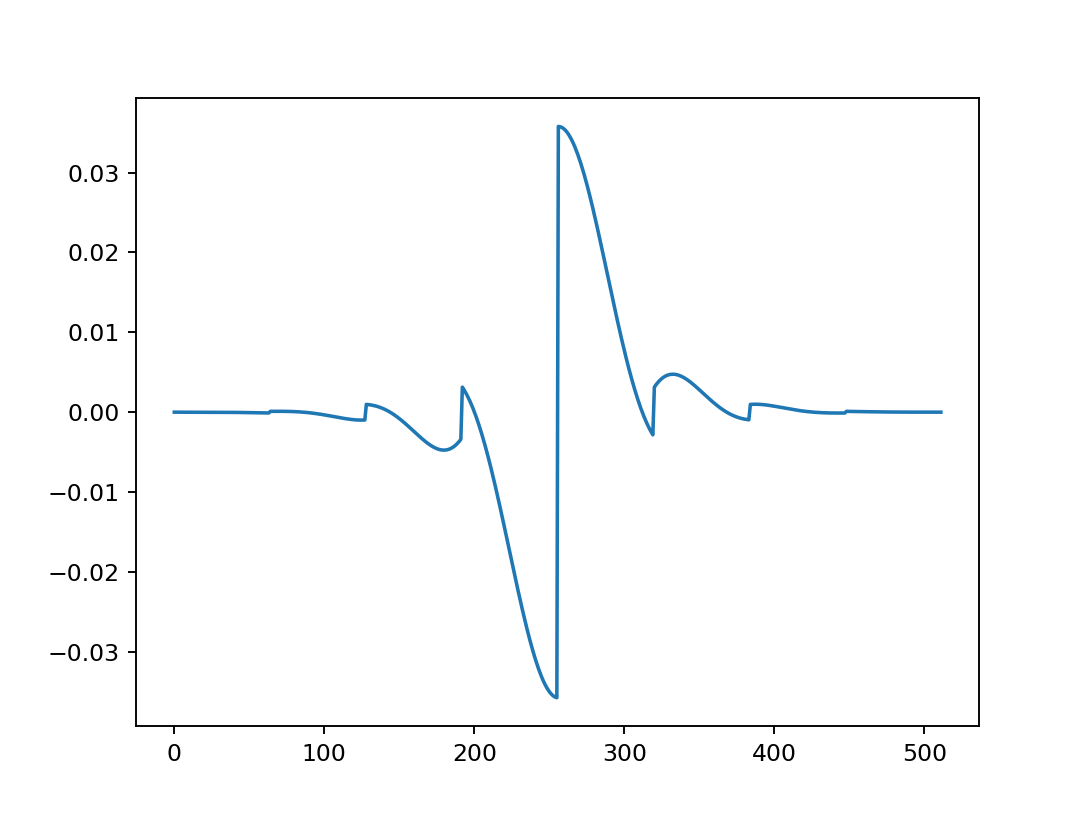
\includegraphics[width=0.6\textwidth]{analysis/c_taps}
	\caption{Plot of a 512 tap analysis filter, $C$, used in MP3 encoding.}
	\label{fig:c_taps}
\end{figure}

Let us define (see Fig. \ref{fig:c_taps}),

\begin{equation}
c(m) = 
	\begin{dcases}
		p_0(m) &\text{if $q=\lfloor m/64 \rfloor$ is even} \\
		-p_0(m) &\text{if $q=\lfloor m/64 \rfloor$ is odd},
	\end{dcases}
\end{equation}

then

\begin{equation}
h_k(64q+r) = c(64q+r)cos\left(\frac{(2k + 1) (r - 16)\pi}{64} \right).
\end{equation}

\pagebreak

Using the notation of the MP3 standard, we define

\begin{equation}
\boxed{M_{k,r} = cos\left(\frac{(2k + 1) (r - 16)\pi}{64} \right), \quad k=0,...,31, \quad r=0,...,64,}
\end{equation}

so,

\begin{equation}
h_k(64q+r) = c(64q+r)M_{k,r},
\end{equation}

and

\begin{equation} \label{eq:fast_analysis_output}
s_k(n) = \sum_{q=0}^7 \sum_{r=0}^{63} M_{k,r} c(64q+r)x(32n-64q-r)
\end{equation}

Expressing the analysis in the form of \eqref{eq:fast_analysis_output}, we can efficiently compute sub-band sample coefficients. For every $n$, we compute:

\begin{equation} \label{eq:z}
z(64q+r) = c(64q+r)x(32n-64-r), \quad r = 0,...,63, \quad q = 0,...,7,
\end{equation}

sum over $q$

\begin{equation} \label{eq:y}
y(r) = \sum_{q=0}^7 z(64q+r), \quad r=0,...,63,
\end{equation}

and compute one sample output for each sub-band by taking a sum over $r$

\begin{equation} \label{eq:s}
s_k = \sum_{r=0}^{63} M_{k,r} y(r), \quad	k=0,...,31.
\end{equation}

\subsection{Frequency inversion}
Downsampling has the effect of moving the output of each filter down to the baseband. However, the periodic nature of the discrete-time Fourier transform (DTFT) representation, causes a "frequency inversion" to occur, where higher frequency components appear to be to the left of the y-axis. This can be illustrated visually in Fig. \ref{fig:inversion}.

\begin{figure}[ht]
	\centering
	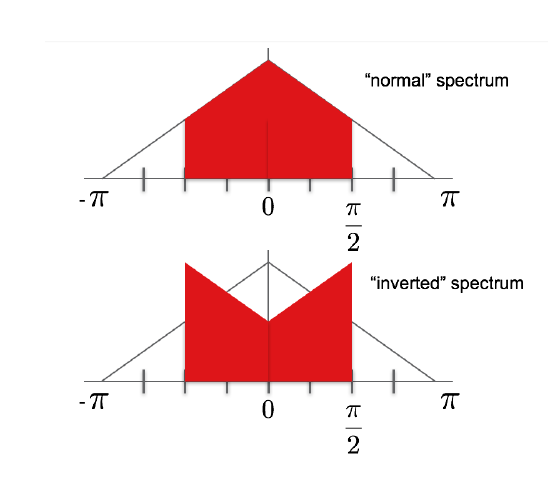
\includegraphics[width=0.6\textwidth]{analysis/freq_inversion}
	\caption{Spectrum inversion}
	\label{fig:inversion}
\end{figure}

Considering the first sub-band filter to be index 0, then as it works out, the \textit{odd} sub-bands are inverted. The MP3 codec further decomposes the filter bank output using the modified discrete cosine transform (MDCT), so it is desirable to undo the inversion. In complex exponential form, this can be accomplished by multiplying the signal by $e^{j\pi n}$, but in Python and other analysis tools where only the exponential coefficients are considered, we can simply multiply the sample output of every odd sub-band by -1. This operation has the effect of translating the spectral signal by $\pi$, restoring its orientation because the DTFT is periodic in $2\pi$.

\pagebreak

\subsection{Implementation}
Our analysis was done in Python, however the basic procedure of implementation will be the same for any implementation.

Each processing cycle works on packets of 32 audio samples and the filtering is performed on a buffer $X$ of size 512. The buffer is shifted to the right by 32 samples and the available indexes at the left end of the buffer are filled with new audio samples. 32 sub-band coefficients are computed and this process is repeated until the length of the input signal is reached.

In this lab, the window filter coefficients, $c$, were calculated prior and provided in the form of a text file. The 512 coefficients were read into a \verb|numpy| array at the beginning of analysis to be used in calculation later. Audio was provided as \verb|.wav| tracks. We used \verb|scipy.io.wavfile.read()| to convert these files to \verb|numpy| arrays. Further analysis was performed on the first 5 seconds of each track.

\begin{figure}[ht]
	\centering
	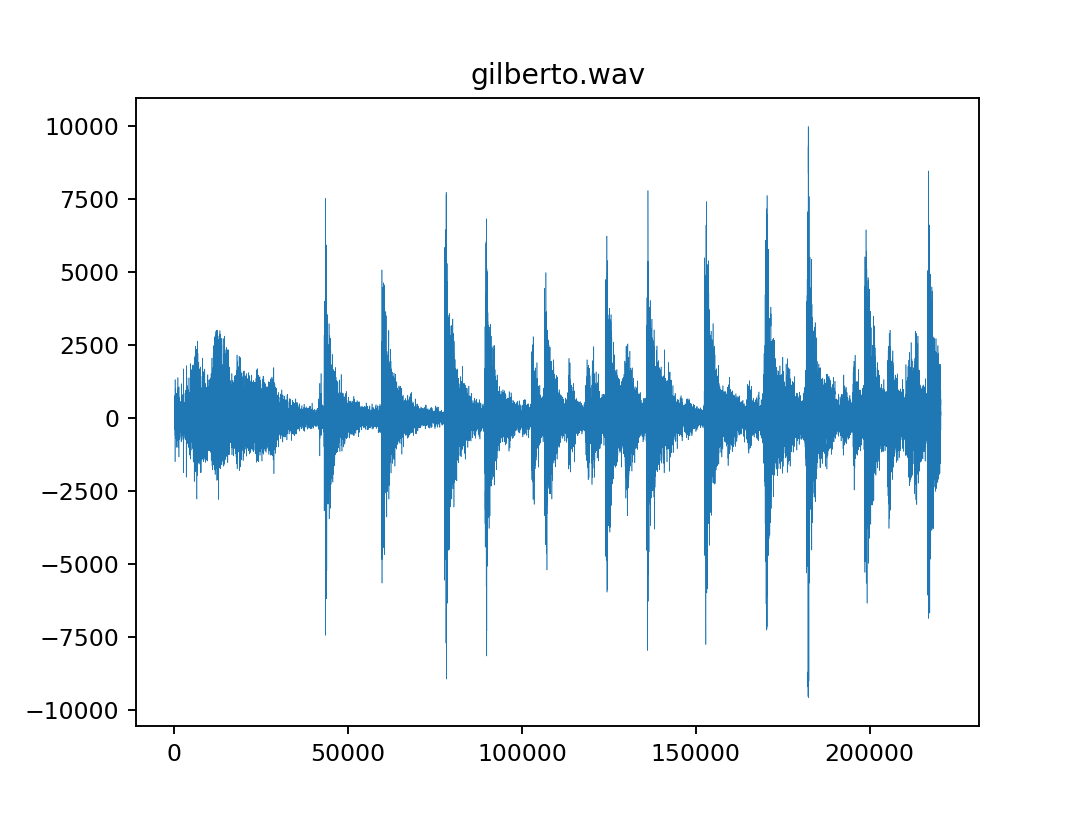
\includegraphics[width=0.65\textwidth]{gilberto}
	\caption{Plot of samples vs. magnitude for first 5 seconds of a jazz song, used as input to our analysis.}
	\label{fig:gilberto}
\end{figure}

\clearpage

We begin calculation of sub-band coefficients by reshaping the audio sample array to have dimension (-1,32), where -1 means the first dimension is implied. I implemented a quick calculation to append zeros to the end of the array if it did not have the correct number of elements to be reshaped directly. Before beginning to loop over the rows of this new matrix of audio samples, we can build $M$ one time to save processing cycles. A temporary buffer, $X$ of length 512, an output matrix of \verb|np.zeros_like| the (-1,32) input sample data, and a couple helper vectors which allow vector operations instead of sums, are all declared outside of the loop. One helper vector, \verb|fInvert| is used for frequency inversion correction. 

\begin{align*}
fInvert = [1, -1, 1, \ldots, 1] \quad &\text{length = } 32
\end{align*}

As well as \verb|zFlat|, a length 8 vector of ones which replaces the sum in \eqref{eq:y}.

Now for the actual analysis. We loop over each row, effectively performing operations on a "packet" of 32 samples for each loop iteration. For each packet,

\begin{enumerate}
\item Shift every value in buffer $X$ right by 32
\item Fill X[0:32] with packet (flipped to perform convolution)
\item Compute $Z = C * X$, windowing X by the analysis filter taps (eq. \eqref{eq:z})
\item Reshape $Z$ into (8,64) and calculate $Y = zFlat \cdot Z$ (eq. \eqref{eq:y})
\item Compute $S = M \cdot Y$ (eq. \eqref{eq:s})
\item Store length 32 output vector, $S$ in a row of output matrix
\end{enumerate}

The output of this sequence should be a matrix of sub-band coefficients organized like so (input matrix of shape (N,32)):

\begin{equation}
A = 
	\begin{bmatrix}
		sb_{0,0} & sb_{0,1} & sb_{0,2} & \ldots & sb_{0,31} \\
		sb_{1,0} & sb_{1,1} & sb_{1,2} & \ldots & sb_{1,31} \\
		\ldots \\
		sb_{N,0} & sb_{N,1} & sb_{N,2} & \ldots & sb_{N,31} \\
	\end{bmatrix}
\end{equation}

and will also have shape (N,32).

Transposing and flattening $A$, we can plot the sub-band analysis output.

\clearpage

\begin{figure}[ht]
	\centering
	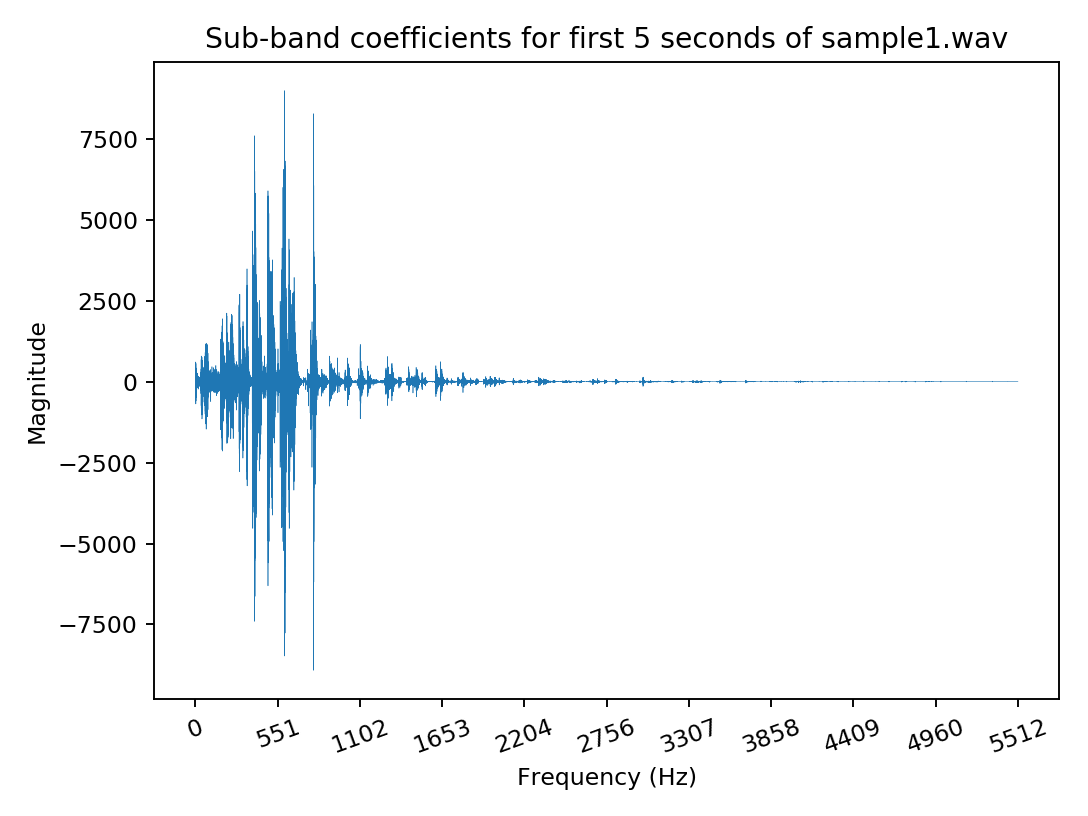
\includegraphics[width=0.65\textwidth]{analysis/sample1}
	\caption{Spectral content of a piano melody. We see a small magnitude of very low frequencies, most of the energy concentrated in the low-mid frequency range, and almost no content at high frequency.}
	\label{fig:analysis_sample1}
\end{figure}

\begin{figure}[ht]
	\centering
	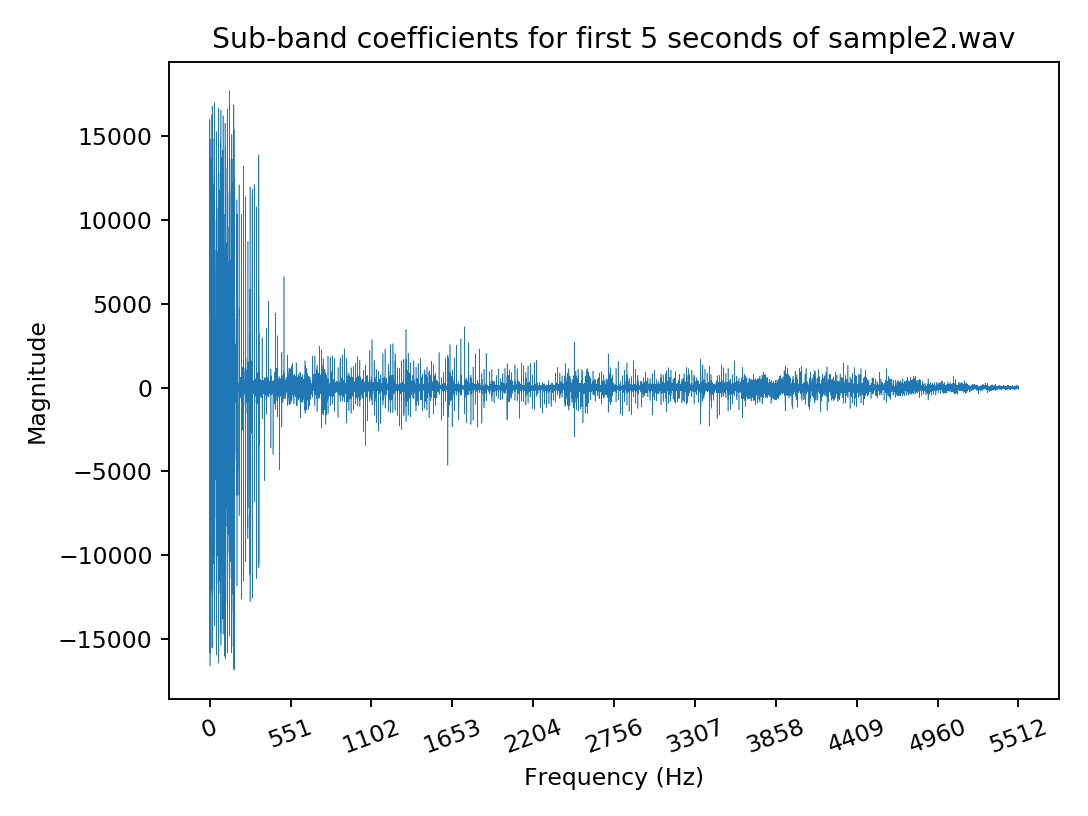
\includegraphics[width=0.65\textwidth]{analysis/sample2}
	\caption{Spectral content of a dance floor beat. We see high energy density at very low frequencies and lots of noise at higher frequencies.}
	\label{fig:analysis_sample2}
\end{figure}

\clearpage

\begin{figure}[ht]
	\centering
	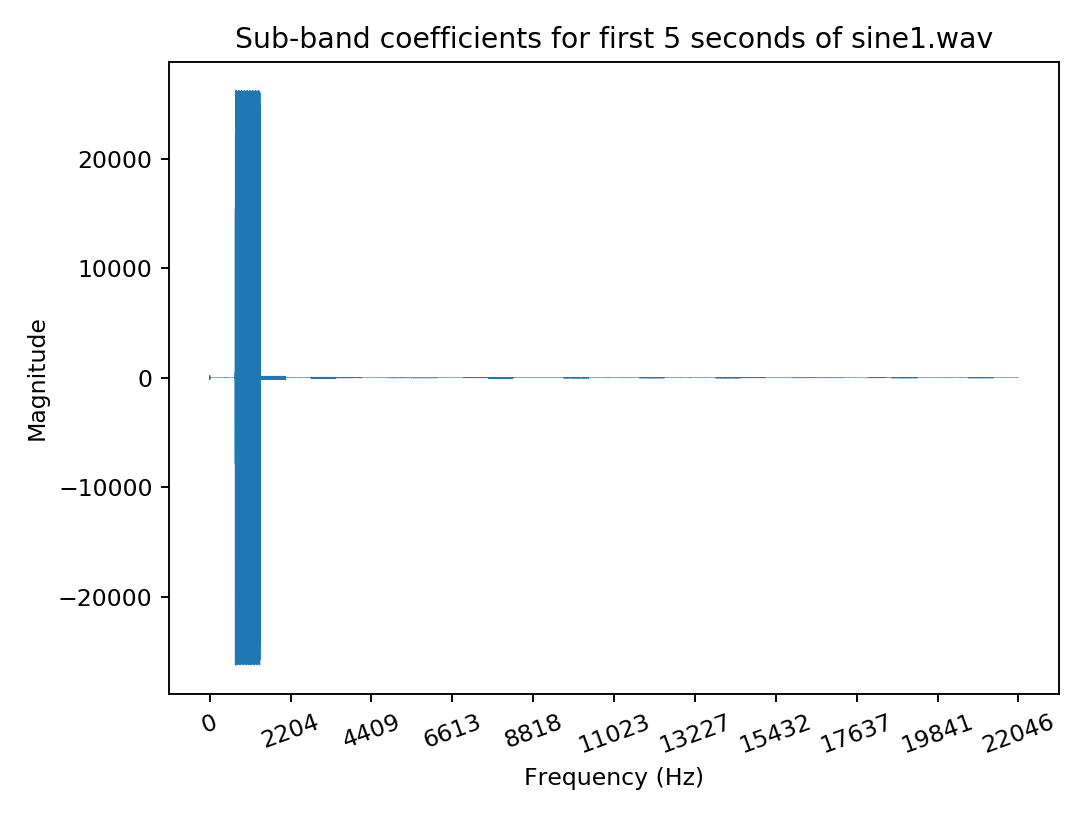
\includegraphics[width=0.65\textwidth]{analysis/sine1}
	\caption{Spectral content of a sine wave. We see energy only between about 750 Hz and 1250 Hz.}
	\label{fig:analysis_sine1}
\end{figure}

\begin{figure}[ht]
	\centering
	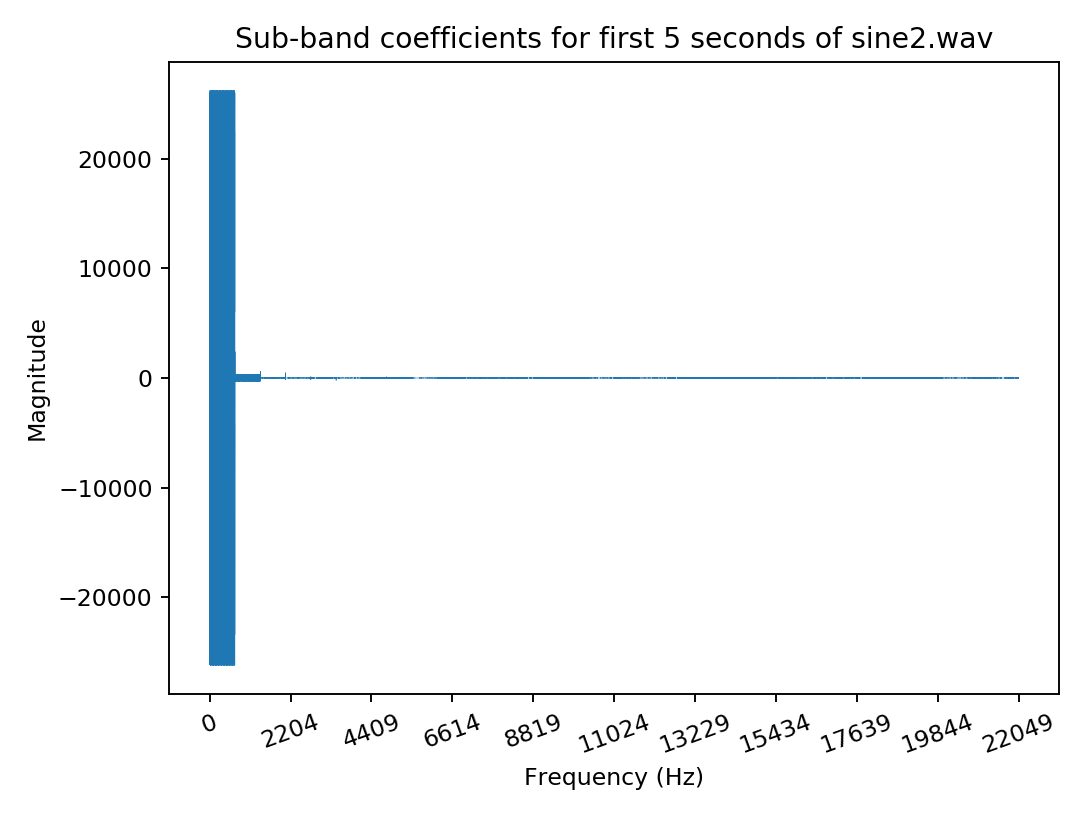
\includegraphics[width=0.65\textwidth]{analysis/sine2}
	\caption{Spectral content of a sine wave. We see energy only between 0 Hz and 750 Hz.}
	\label{fig:analysis_sine2}
\end{figure}

\clearpage

\begin{figure}[ht]
	\centering
	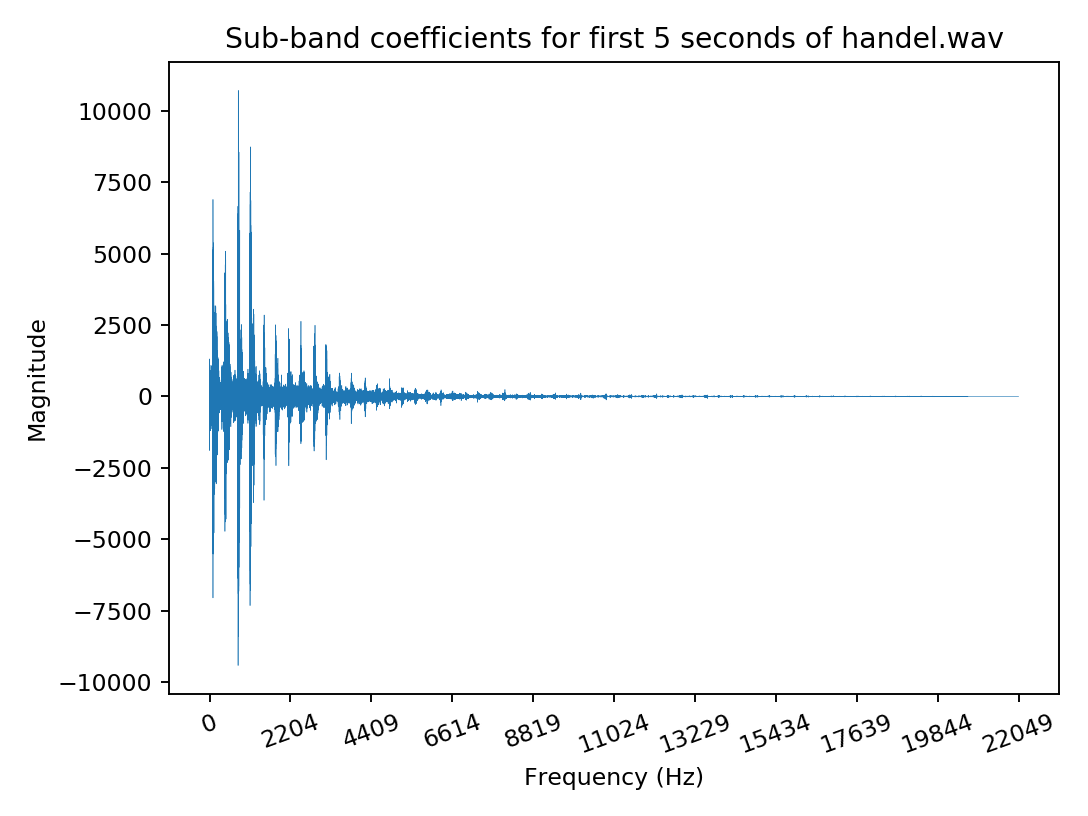
\includegraphics[width=0.65\textwidth]{analysis/handel}
	\caption{Spectral content of a classical track. There is good contribution from spectral bands at 0 Hz all the way up to about 5 kHz.}
	\label{fig:analysis_handel}
\end{figure}

\begin{figure}[ht]
	\centering
	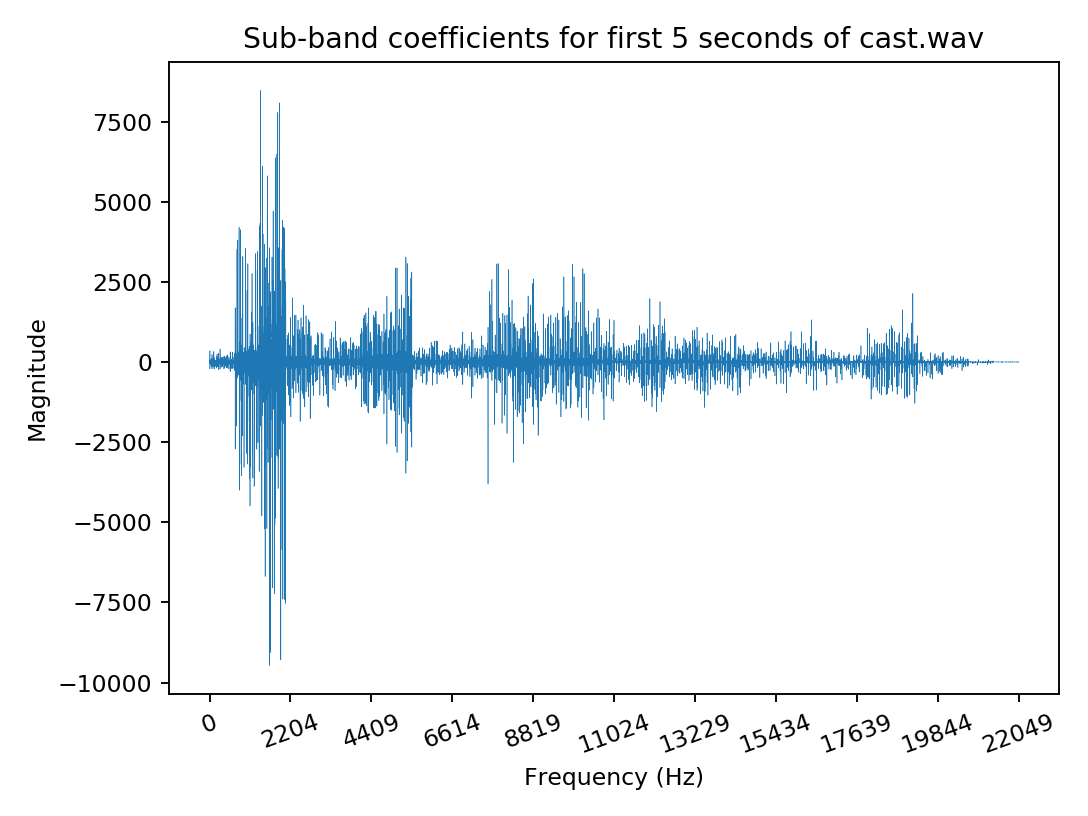
\includegraphics[width=0.65\textwidth]{analysis/cast}
	\caption{Spectral content of a percussive recording. The energy is distributed fairly evenly across the frequency spectrum here.}
	\label{fig:analysis_cast}
\end{figure}

\clearpage

\begin{figure}[ht]
	\centering
	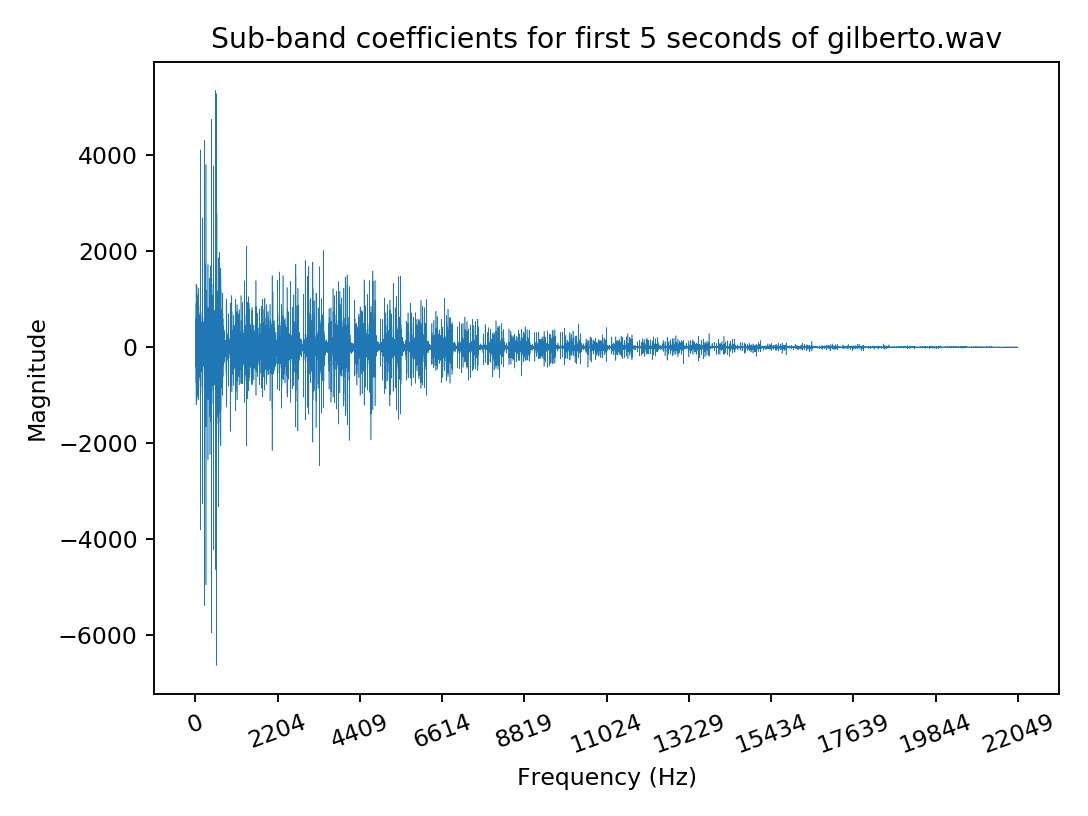
\includegraphics[width=0.65\textwidth]{analysis/gilberto}
	\caption{Spectral content of a jazz track. The first five seconds are very percussion heavy, most likely leading to the large spread of spectral content. Above about 16 kHz there is mostly noise.}
	\label{fig:analysis_gilberto}
\end{figure}

\pagebreak

\section{Reconstruction: Synthesis}
Synthesis, or reconstruction of the MP3 codec is very similar to analysis. For each set of 32 sub-band coefficients, 32 audio samples are reconstructed. The algorithm will need to reverse the frequency inversion correction, so we will actually invert the signal again.

\subsection{Calculations}

This time, we will perform modulation with a matrix $N$ where,

\begin{equation}
N_{i,k} = cos\left(\frac{(2k+1)(16+i)\pi}{64} \right), \quad i = 0,...,63, \quad k=0,...,31.
\end{equation}

First, we load reconstruction filter tap coefficients from a text file to obtain the window in Fig. \ref{fig:d_taps}

\begin{figure}[ht]
	\centering
	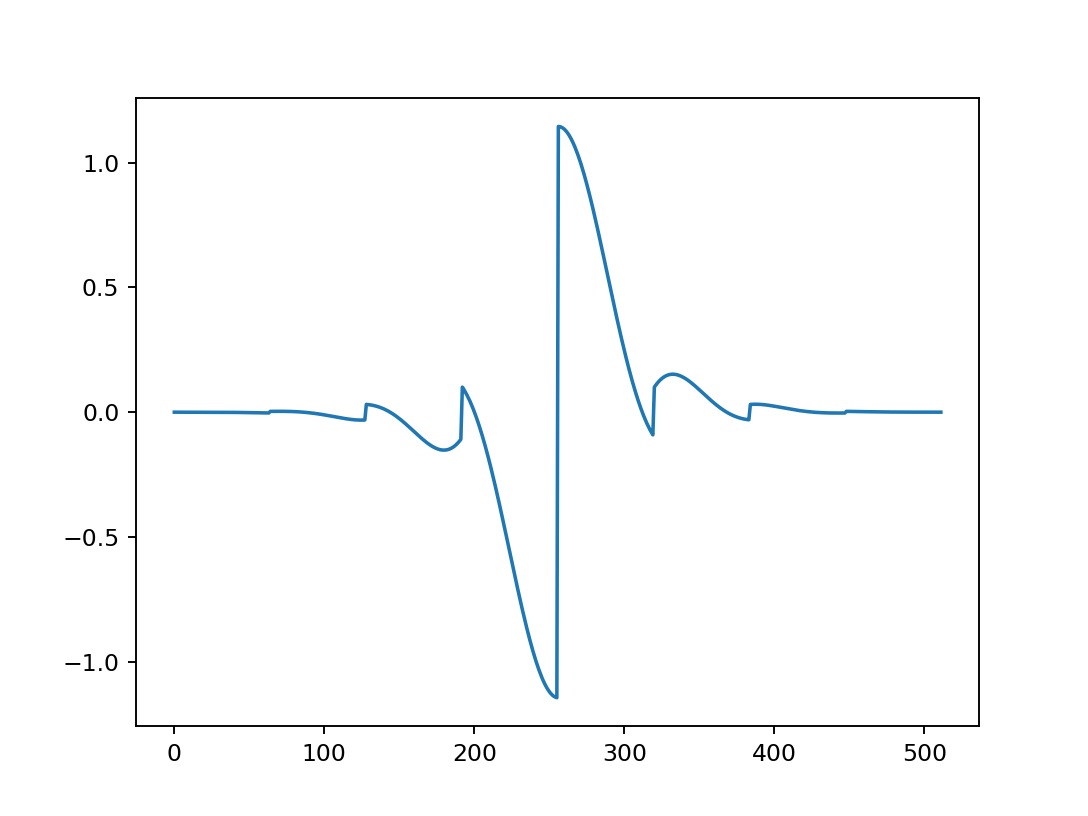
\includegraphics[width=0.5\textwidth]{synthesis/d_taps}
	\caption{Plot of reconstruction window $D$.}
	\label{fig:d_taps}
\end{figure}

We again operate on "packets" of length 32 samples and loop over vectors of this length through to the end of the track. This time our buffer vector $V$ is of length 1024, we declare length 512 vectors $U$ and $W$, an output vector $S$ and two more helping vectors, \verb|fInvert| as before and a length 16 vector of ones, \verb|wFlat|.

We will build U during each cycle and use it to compute the reconstruction. $V$ is constructed over multiple packet cycles and so the content of $U$ is also updated. We define

\begin{figure}[ht]
	\centering
	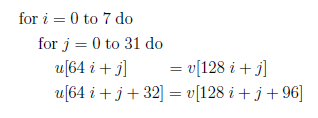
\includegraphics[scale=1]{synthesis/u_vect}
\end{figure}

\subsection{Implementation}

The steps in reconstruction go as follows:

\begin{enumerate}
\item Shift every value in a buffer $V$ right by 64
\item Calculate modulation and re-invert: $V[0:64] = N \cdot (fInvert * packet)$
\item Compute $U$ as shown above
\item Window the samples vector by $W = U * D$
\item Reshape $W$ into (16,-1) and store $wFlat \cdot W$ in output matrix
\end{enumerate}

Plotting the output of this reconstruction procedure, we can compare it to the original signal.

\begin{figure}[ht]
	\centering
	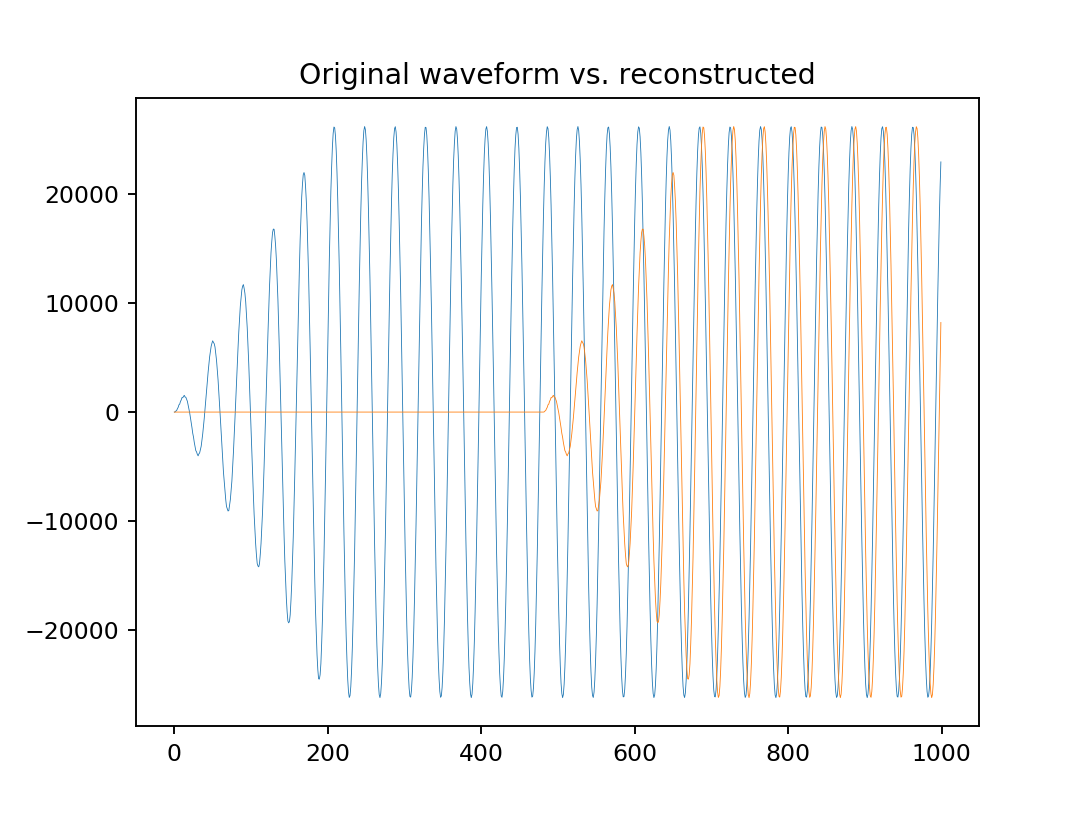
\includegraphics[width=0.75\textwidth]{synthesis/sine1_delay}
	\caption{Plot of first 1000 samples of a simple sine wave input signal, sine1.wav. Observe the reconstructed signal is delayed by some amount. \\ error = 2.62}
	\label{fig:delay}
\end{figure}

Through trial and error, attempting to minimize the error between the original signal and reconstruction, I found the delay to be equal to 481 samples. This is caused by having an empty buffer when we begin synthesis. The it is only after 15 packets of information, that the buffer is full (with 512 values) and so the first 15 cycles produce a delay of available information. We start with 32 samples and index from 0, thus we have a delay of 481 samples.

\begin{figure}[ht]
	\centering
	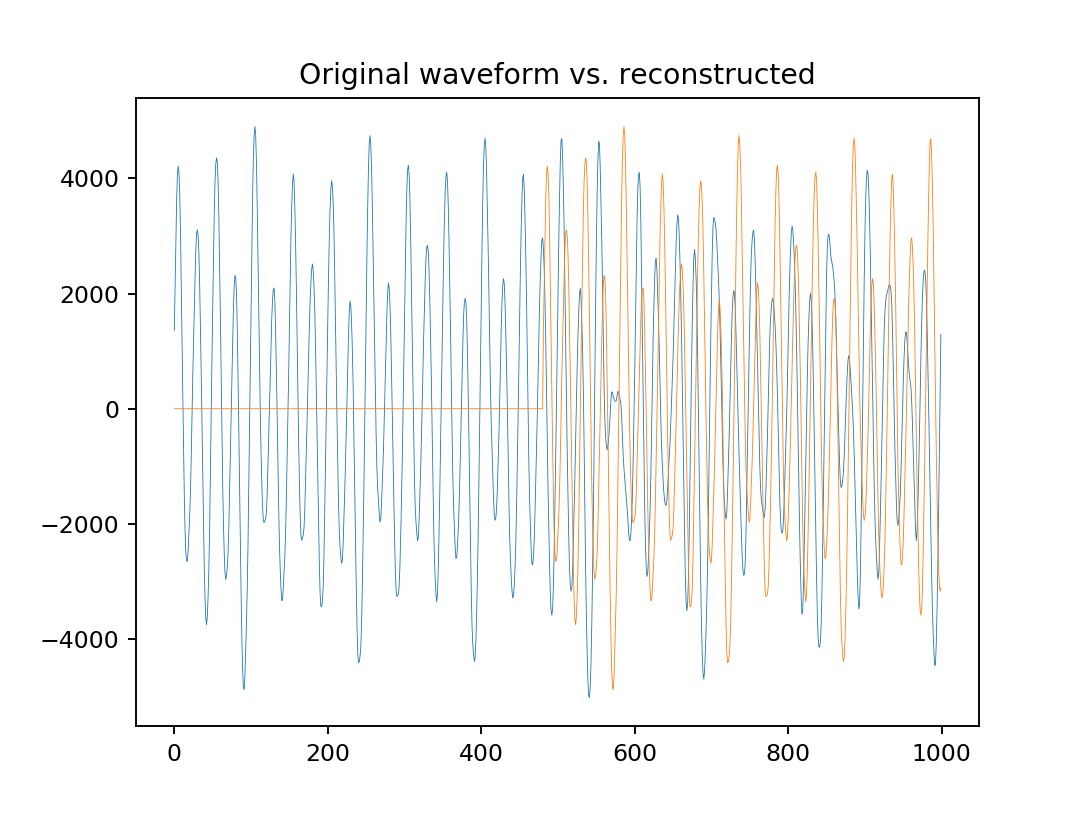
\includegraphics[width=0.75\textwidth]{synthesis/sample1_delay}
	\caption{Reconstruction and delay shown for sample1.wav \\ error = 0.24}
	\label{fig:synthesis_sample1}
\end{figure}

\begin{figure}[ht]
	\centering
	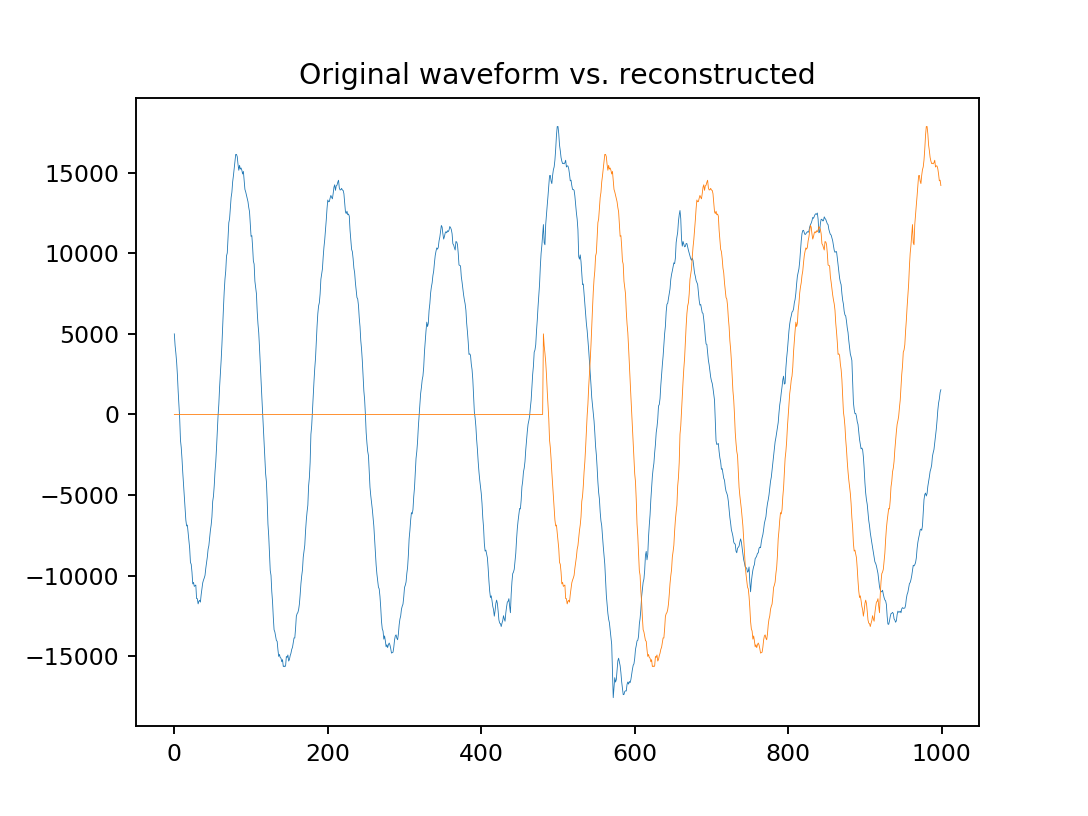
\includegraphics[width=0.75\textwidth]{synthesis/sample2_delay}
	\caption{Reconstruction and delay shown for sample2.wav \\ error = 1.32}
	\label{fig:synthesis_sample2}
\end{figure}

\pagebreak

\begin{figure}[ht]
	\centering
	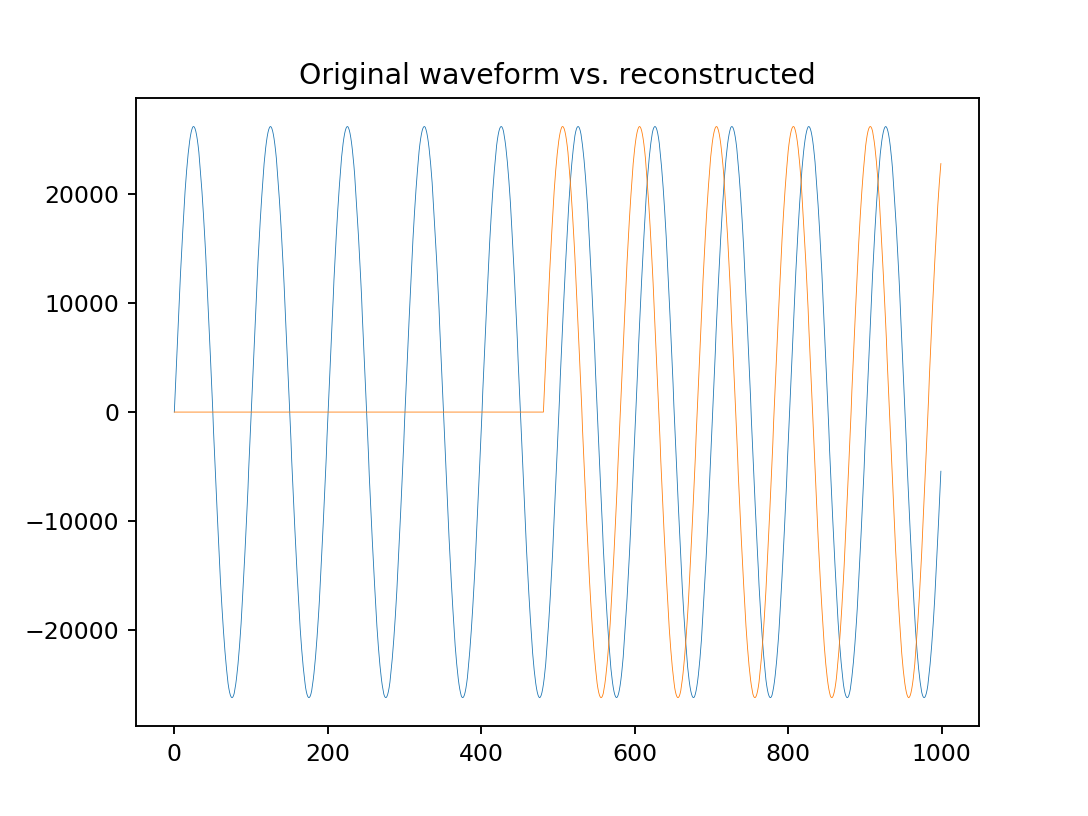
\includegraphics[width=0.75\textwidth]{synthesis/sine2_delay}
	\caption{Reconstruction and delay shown for sine2.wav \\ error = 1.47}
	\label{fig:synthesis_sine2}
\end{figure}

\begin{figure}[ht]
	\centering
	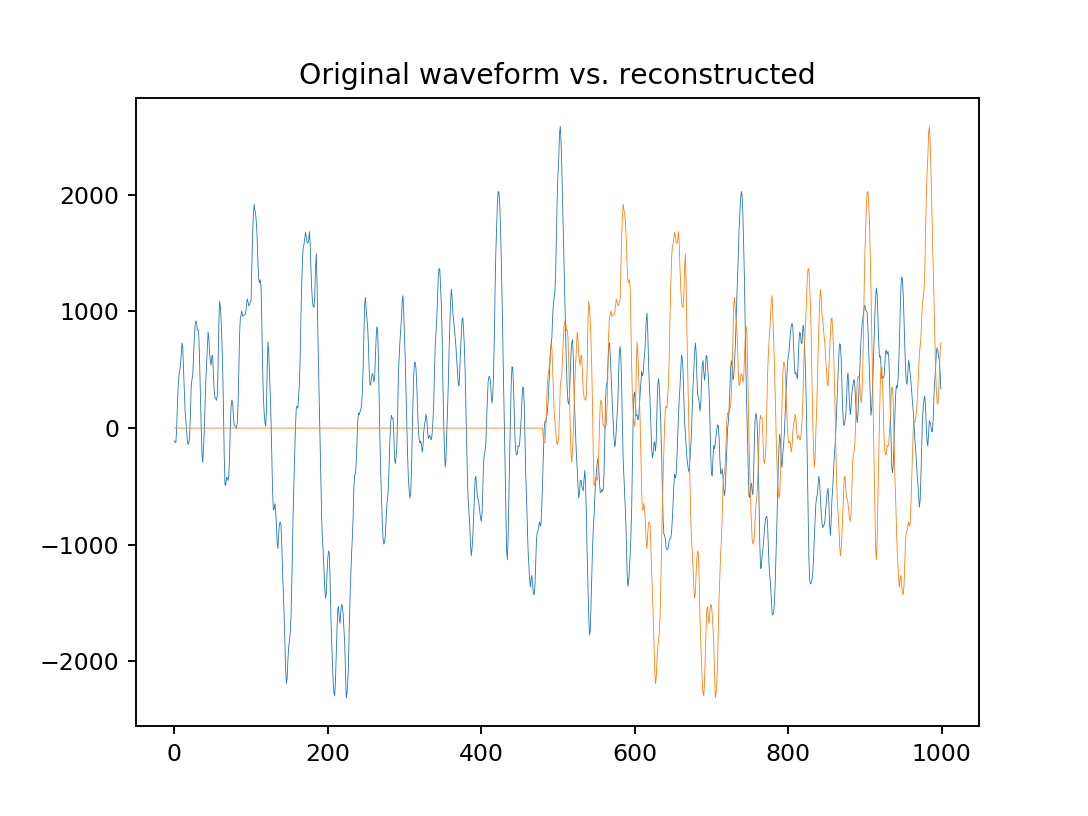
\includegraphics[width=0.75\textwidth]{synthesis/handel_delay}
	\caption{Reconstruction and delay shown for handel.wav \\ error = 0.15}
	\label{fig:synthesis_handel}
\end{figure}

\pagebreak

\begin{figure}[ht]
	\centering
	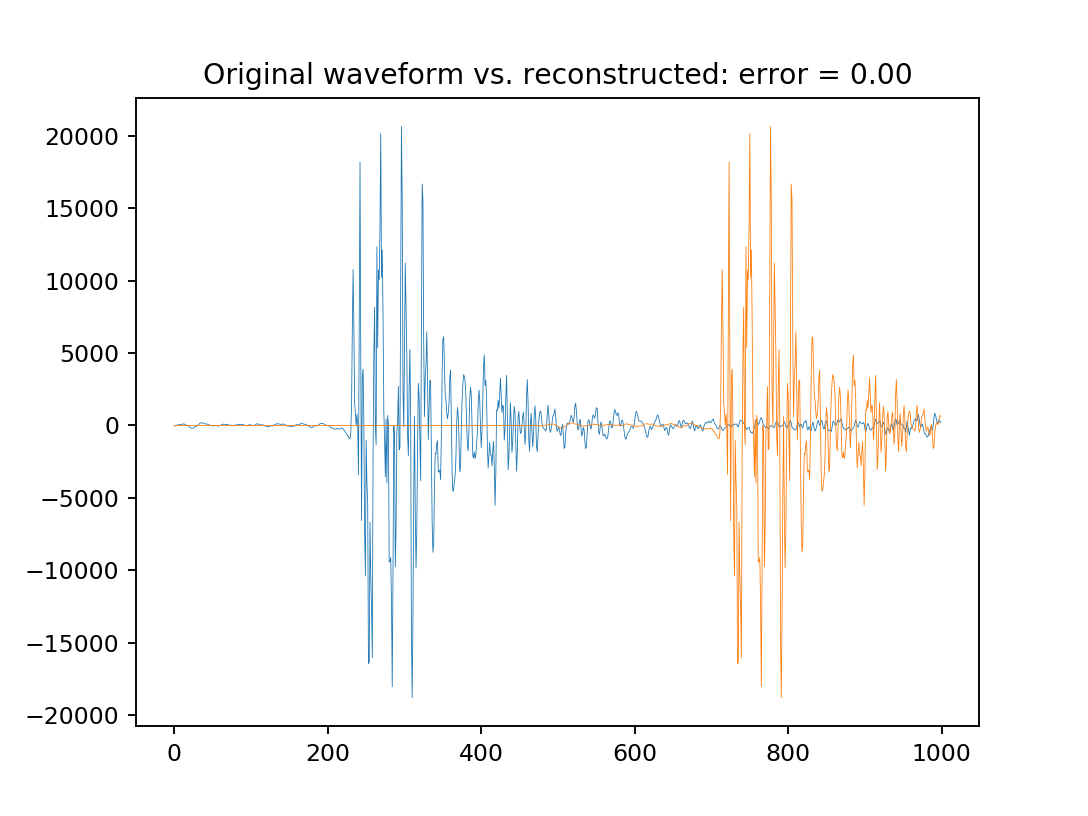
\includegraphics[width=0.75\textwidth]{synthesis/cast_delay}
	\caption{Reconstruction and delay shown for cast.wav \\ error = 0.0}
	\label{fig:synthesis_cast}
\end{figure}

\begin{figure}[ht]
	\centering
	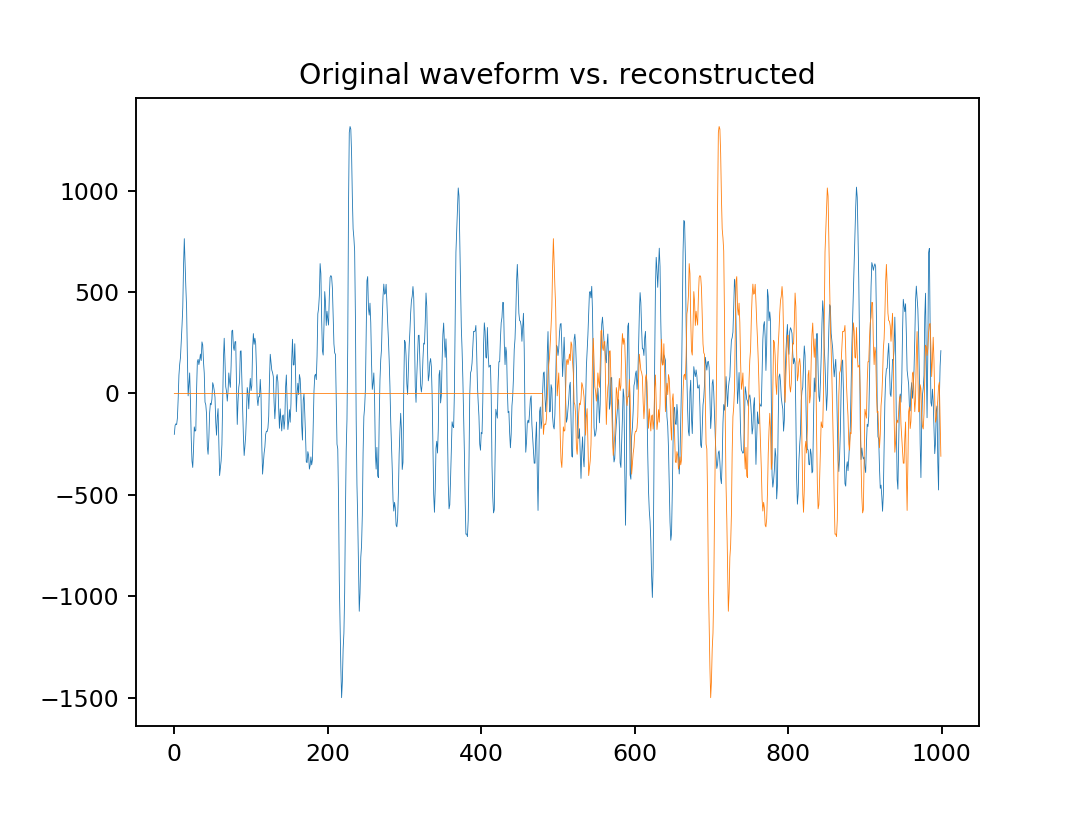
\includegraphics[width=0.75\textwidth]{synthesis/gilberto_delay}
	\caption{Reconstruction and delay shown for gilberto.wav \\ error = 0.065}
	\label{fig:synthesis_gilberto}
\end{figure}

\clearpage

The errors listed in each of the figures above are calculated as maximum error between the original samples and reconstructed samples for only the first 1000 samples. It is scaled based on the maximum sample value in each song, so the values appear much larger than they are if the data were normalized.

\subsection{Selective sub-bands}
Since MP3 is a compression algorithm, we are interested in reconstructing partial data less than perfectly. In the MP3 codec, this is implemented by applying a psychoacoustic model to select a subset of the 32 sub-bands based on human auditory sensitivity. For this lab, we will manually select some bands to leave out, attempting to limit the data used to reconstruct without negatively affecting the perception of music.

For some tracks this is trivial, while for others it is a more complicated task. We will define a compression to be

\begin{equation}
\frac{\text{number of bands used to reconstruct}}{32}
\end{equation}

Selecting bands only where the frequency has large magnitude, the error was calculated as follows for each track:

\begin{align*}
cast &= 0.83 \\
gilberto &= 229.88 \\
handel &= 164.11 \\
sample1 &= 115.99 \\
sample2 &= 10376.86 \\
sine1 &= 789.02 \\
sine2 &= 6735.96
\end{align*}

Again, these errors are not scaled to normalization and a few are probably much larger than ideal, but this was not very analytic.

\section{Conclusion}
This lab was conceptually much more difficult than the previous labs and the code was really nothing new. I did learn a lot more about the DFT, DTFT, frequency analysis in general, and how all of that can be implemented in software. I feel like my foundation of Fourier analysis is much stronger now. This was a cool introduction to a real compression scheme.

\pagebreak

\section{Appendix}

\subsection{PQMF}
\begin{lstlisting}[language=Python]
def pqmf(input):

    # load window coefficients from file
    c_taps = load_c_taps('the_c_taps.txt')

    plt.figure(dpi=170)
    plt.plot(c_taps)
    plt.savefig('./figures/analysis/c_taps.png')
    plt.close()

    # add zeros at end of array to make it reshapable into 32 cols
    data = np.append(input, np.zeros(32 - (len(input) % 32)))
    # reshape into 32 sample length rows
    data = np.reshape(data, (-1, 32))

    # initialize working arrays for subband coefficient calculation
    X = np.zeros(512)

    # build filter matrix, M
    M = np.zeros([32, 64])
    for k in range(32):
        for r in range(64):
            M[k,r] = math.cos((( (2 * k) + 1) * (r - 16) * math.pi) / 64)

    # subband coefficient output matrix
    A = np.zeros_like(data)

    # helping vectors
    fInvert = np.array(16 * [1, -1])
    zFlat = np.array(8 * [1])

    # loop over entire song in 32 sample chunks
    for packet in range(np.shape(data)[0]):
        # shift every element of X to the right by 32
        X = np.roll(X, 32)
        # flip audio sample frame and place in X
        X[0:32] = np.flip(data[packet])
        # window X by C filter
        Z = c_taps * X
        # partial calculation
        Z = np.reshape(Z, (8, 64))
        Y = zFlat.dot(Z)
        # calculate 32 subband samples
        S = M.dot(Y)
        # undo frequency inversion and add to output array
        A[packet, :] = fInvert * S

    return A
\end{lstlisting}

\pagebreak

\subsection{IPQMF}
\begin{lstlisting}[language=Python]
def ipqmf(input, subbands):

    data = input

    # load window coefficients from file
    d_taps = load_d_taps('the_d_taps.txt')

    plt.figure(dpi=170)
    plt.plot(d_taps)
    plt.savefig('./figures/synthesis/d_taps.png')
    plt.close()

    # declare working array
    V = np.zeros(1024)
    U = np.zeros(512)
    W = np.zeros(512)

    # reconstruction coefficient output matrix
    S = np.zeros_like(data)

    # build reconstruction matrix, N
    N = np.zeros([64, 32])
    for i in range(64):
        for k in range(32):
            N[i,k] = math.cos((( (2 * k) + 1) * (16 + i) * math.pi) / 64)

    # helping vectors
    fInvert = np.array(16 * [1, -1])
    wFlat = np.array(16 * [1])

    # loop over coefficients in 32 sample chunks
    for packet in range(np.shape(data)[0]):
        # filter output sub-bands
        data[packet] = data[packet]
        # shift every element of V to the right by 64
        V = np.roll(V, 64)
        # compute reconstruction samples
        V[0:64] = N.dot(fInvert * data[packet] * subbands)
        # build window operand
        for i in range(8):
            for j in range(32):
                U[i * 64 + j] = V[i * 128 + j]
                U[i * 64 + 32 + j] = V[i * 128 + 96 + j]
        # window
        W = U * d_taps
        W = np.reshape(W, (16, -1))
        S[packet, :] = wFlat.dot(W)

    return S
\end{lstlisting}

\pagebreak

\subsection{Main}
\begin{lstlisting}[language=Python]
import lab04_funcs as lf
from tkinter import filedialog
import numpy as np
import scipy.io.wavfile
import matplotlib.pyplot as plt

d_taps = lf.load_d_taps('the_d_taps.txt')

# UI dialog to select files -> selection of multiple files will run all functions for each file
files = filedialog.askopenfilenames()
# Loop over files selected
for f in files:
    filename = str.split(f,'/')[-1]
    filename = str.split(filename,'.')[0]
    filepath = f

    # read .wav file into numpy array and extract sampling frequency
    fs, data = scipy.io.wavfile.read(filepath)
    
    # extract first 5 seconds of .wav file
    data = data[0 : int(5 * fs)]

    # plot input samples
    plt.figure(dpi=170)
    plt.plot(data, linewidth=0.25)
    plt.title(filename + '.wav')
    plt.savefig('./figures/' + filename + '.png')
    plt.close()

    # calculate sub-band filter coefficients
    print('Analyzing ' + filename + ' ... \n')
    coefficients = lf.pqmf(data)

    # vector to filter subbands
    thebands = np.ones(32)

    # calculate reconstruction coefficients
    print('Reconstructing ' + filename + ' ...\n')
    recons = lf.ipqmf(coefficients, thebands)

    # transpose and flatten to sort data into incrementing groups of subband coefficients
    coefficients = coefficients.T.flatten()

    # plot sub-band coefficients
    plt.figure(dpi=170)
    plt.plot(coefficients, linewidth=0.25)
    xlocs = np.asarray(range(0, len(coefficients), int(len(coefficients)/10)))
    xvals = np.asarray(xlocs/np.amax(range(len(coefficients)))*fs/2, int)
    plt.xticks(xlocs, xvals, rotation=20)
    plt.xlabel('Frequency (Hz)')
    plt.ylabel('Magnitude')
    plt.title('Sub-band coefficients for first 5 seconds of ' + filename + '.wav')
    plt.tight_layout()
    plt.savefig('./figures/analysis/' + filename + '.png')
    plt.close()

    recons = recons.flatten()
    
    # plot reconstruction coefficients
    plt.figure(dpi=170)
    plt.plot(recons, linewidth=0.25)
    plt.xlabel('Sample')
    plt.ylabel('Magnitude')
    plt.title('Reconstruction of first 5 seconds of ' + filename + '.wav')
    #plt.show()
    plt.savefig('./figures/synthesis/' + filename + '.png')
    plt.close()

    delay = 512 - 31;

    # calculate error
    r = recons[delay:1000 + delay]
    d = data[0:1000]
    error = np.amax(r - d)
    print(filename + f' error = {error}')

    # plot delay
    plt.figure(dpi=170)
    plt.plot(data[0:1000], linewidth=0.35)
    plt.plot(recons[0:1000], linewidth=0.35)
    if (filename == 'cast'):
        plt.clf()
        plt.plot(data[2850:3850], linewidth=0.35)
        plt.plot(recons[2850:3850], linewidth=0.35)
    plt.title('Original waveform vs. reconstructed')
    plt.savefig('./figures/synthesis/' + filename + '_delay.png')
    plt.close()
    
    thebands = np.ones(32)
    coefficients = np.reshape(coefficients, (32, -1)).T
    if filename == 'gilberto':
        thebands[16:32] = 0
    elif filename == 'sine1':
        thebands[0] = 0
        thebands[2:32] = 0
    elif filename == 'sine2':
        thebands[1:32] = 0
    elif filename == 'handel':
        thebands[8:32] = 0
    elif filename == 'sample1':
        thebands[8:32] = 0
    elif filename == 'sample2':
        thebands[15:32] = 0
    selective_output = lf.ipqmf(coefficients, thebands)
    selective_output = selective_output.flatten()
    # calculate error
    r = selective_output[delay:delay + 5000]
    d = data[0:5000]
    error = np.amax(r - d)
    print(filename + f' selective error = {error}')


print('done')

\end{lstlisting}

\end{document}